\begin{figure}[!h]
  \begin{center}
    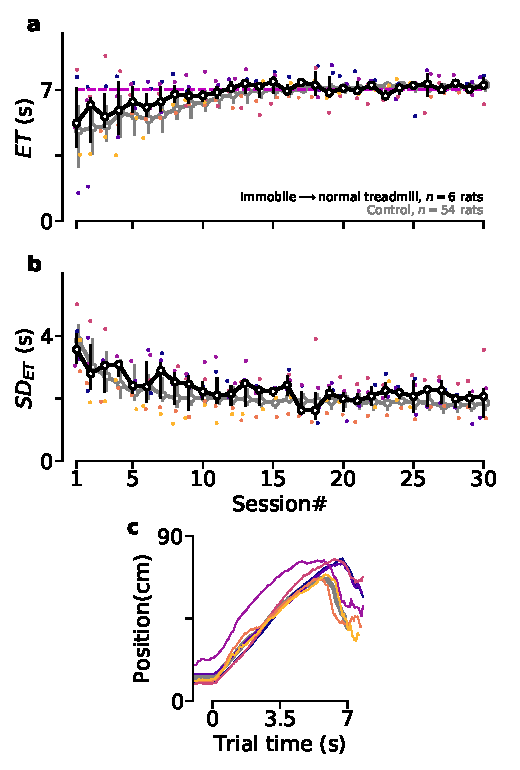
\includegraphics[scale=1]{ch-appendicies/figures/Imm2CtrlTrd.pdf}
    \caption[Immobile Animals Relearning the Task]
    {\textbf{Lack of temporal knowledge transfer across task protocols.}
    After extensive training on the immobile treadmill, animals were trained under normal conditions (GT$=7$~s, treadmill speed$=10$~cm/s).
    \textbf{a)}
    Median ET across sessions under control condition.
    \textbf{b)}
    Similar to panel~a, for the standard deviation of entrance times ($SD_{ET}$).
    \textbf{c)}
    Median trajectory of the individual animals after relearning the task under the control condition.
    \textbf{a-c)}
    Individual animal color code is preserved in all panels.
    }
    \label{fig:appendix:Imm2Ctrl}
  \end{center}
\end{figure}